\documentclass[12pt]{beamer}
\usetheme{Goettingen}
\usepackage[utf8]{inputenc}
\usepackage[english]{babel}
\usepackage{amsmath}
\usepackage{graphicx}
\usepackage{amsfonts}
\usepackage{amssymb}
\usepackage{graphicx}
\author{Robert James}
\title{A study of Interfaces\\ How? Simply add a twist}
%\setbeamercovered{transparent} 
%\setbeamertemplate{navigation symbols}{} 
\logo{SwanseaLogo.png} 
\institute{Swansea University} 
\date{29/05/2015} 
%\subject{} 
\begin{document}

\begin{frame}
\titlepage
\end{frame}

%\begin{frame}
%\tableofcontents
%\end{frame}

\begin{frame}{Objectives}
At the end of this presentation, I will have lead you through the following steps.
\begin{enumerate}
	\item An introduction to the Potts Model
	\item Accessing Thermodynamic quantities
	\item Why do we care about Interfaces
	\item How to add a twist
	\item Project Results
\end{enumerate}

For each of the above steps, I will summarise how they pertain to my project and any further information.

\end{frame}

\section{An Introduction to the Potts Model}
\begin{frame}{History}
\begin{itemize}
	\item Originally proposed as a thesis topic for Renfrey Potts by Cyril Domb (1951).
	\item The Potts Model was originally proposed as a generalisation of the Ising Model (Ising 1925).
	\item The 4 state planar Potts Model is also known as the Ashkin-Teller model who studied 
\end{itemize}
\end{frame}

\begin{frame}{The Q States}
Each state, in 2D, can be visualised as q possible points uniformly distributed around a circle. The angles can be represented as
\begin{equation}
\theta_{n} = \frac{2 \pi n}{Q}
\end{equation}
Each site on the lattice, $s_i$ can take on the values $\left\lbrace 1,...,Q\right\rbrace$.
\end{frame}

\begin{frame}{Hamiltonian}
In this project, the behaviour of the lattice 
\begin{equation}
\mathcal{H} = -J_{p} \sum_{\left(i,j\right)} \delta_{Kr}\left(s_i,s_j\right)
\end{equation}
In this project, to simplify the values being returned, the coupling constant $J_{p}$ is set to 1.

\end{frame}


\section{Accessing Thermodynamic quantities}
\begin{frame}{Thermodynamic Quantities}
It should now be stated that.
\begin{equation}
\beta = \frac{1}{\kappa_{B} T}
\end{equation}

That being said, this project actually sets many constants to be 1 for simplicity. So from now on you can write $\beta$ as.
\begin{equation}
\beta = \frac{1}{T}
\end{equation}

\end{frame}

\begin{frame}{Thermodynamic Quantities}
It can be shown analytically that the Critical point for the Potts Model in the thermodynamic limit can be written as
\begin{equation}
\beta_{c} = \ln{(1+\sqrt{Q})} 
\end{equation}

This is used heavily in the project as a verification tool of the Metropolis algorithm.

\end{frame}


\begin{frame}{Thermodynamic Quantities}
Now that the housekeeping matters have been attended to.

Various thermodynamic quantities have to be measured on the lattice.

Having the Hamiltonian of the model makes the Energy measurement trivial due to the fact it is equivalent to the Total Energy.

The Spontaneous Magnetisation of the Lattice.
\begin{equation}
\mathcal{M} = -\sum_{i}^{V} s_i
\end{equation}

\end{frame}

\begin{frame}{Other Thermodynamic Quantities}
Other Thermodynamic Quantities that I measured from the Lattice include the Specific Heat and the Magnetic Susceptibility.
These can be written as.
\begin{equation}
C = \beta^2 \left[ \left\langle E^2 \right\rangle - \left\langle E \right\rangle^2 \right]
\end{equation}

\begin{equation}
\chi = \beta \left[ \left\langle M^2 \right\rangle - \left\langle M \right\rangle^2 \right]
\end{equation}

\end{frame}

\begin{frame}{Partition Functions}
A general form for the Partition Function
\begin{equation}
Z = \int g(E) e^{-\beta E} dE
\end{equation}
$g(E)$ is the Density of States and the Boltzmann weighting factor $e^{-\beta E}$.

\end{frame}

\begin{frame}{Partition Functions}
Traditional Monte Carlo methods efficiently sample the distribution and easily determine the statistical averages of observables that have Gaussian fluctuations.

An alternative method requires the numerical calculation of the Density of States using the Wang-Landau algorithm which allows the sampling of observable that have non Gaussian fluctuations.


In this project I use the Wang Landau algorithm to numerically reconstruct the Density of States.
\end{frame}

\section{Interfaces}
\begin{frame}{Why do we care about Interfaces}
Interfaces play a large role for various physical phenomena in fields such as Statistical Mechanics, Soft Condensed Matter, Particle Physics and Biology.

In this project, I studied the Free Energy of Topological Excitations of the  Order-Order interfaces in the Potts Model or equivalently the tension in the 't Hooft Loop for SU(N) gauge theories.

\end{frame}

\begin{frame}{How to add a Twist}
To calculate the Partition function of the system in the presence of a topological excitation, we must first ensure that one exists.

The periodic boundary conditions of the system need to be relaxed on one axis.

At an arbitrary point on this axis, the spin states on one side are modified as shown below.
\begin{equation}
s[i][j] = (s[i-1][j] + 1)\% Q
\end{equation}

There is an implementation issue with the above condition.

\end{frame}

\begin{frame}{Calculating the Interface Free Energy}

To calculate the Free Energy of a topological object on a cubic domain of linear size L, you must extract the ratio of the partition functions of the system in the presence of the excitation over the partition function of the periodic lattice.

The Partition function of the system in the presence of the excitation (interface) can be denoted as $\tilde{Z}(L)$ and the Partition function of the Periodic Lattice is simply $Z(L)$.

\begin{equation}
F_I (L) = -log \frac{\tilde{Z}(L)}{Z(L)} - log(L)
\end{equation}

The term $log(L)$ occurs to correct for the fact that the interface can occur at any L positions in the chosen axis.

\end{frame}


\begin{frame}{Calculating the Interface Tension}
Taking the Interface Free Energy the interface tension $\sigma$ is

\begin{equation}
\sigma = \lim_{L \to \infty} \frac{F_I(L)}{L^{D-1}}
\end{equation}

In this project D is restricted to 2.
\end{frame}

\section{Project Results}
\begin{frame}{Metropolis Algorithm}
The use of a traditional Metropolis algorithm to reconstruct the expected behaviours from the various thermodynamic quantities, was the first stage in verifying I had successfully implemented the Potts Model.

\end{frame}

\subsection{Graphical Representation of the Metropolis Algorithm data}

\begin{frame}{Metropolis Energy Plot}
\begin{figure}
\centering
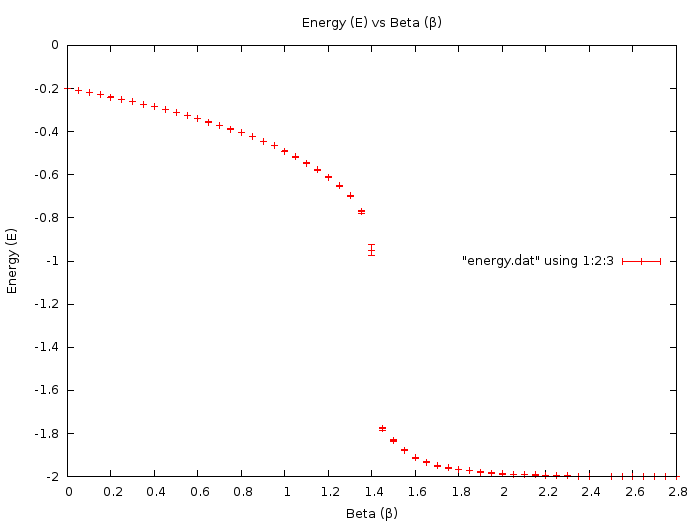
\includegraphics[width=\textwidth]{Q10EnergyBeta16x16RangeofBeta.png}
\end{figure}
\end{frame}

\begin{frame}{Metropolis Magnetisation Plot}
\begin{figure}
\centering
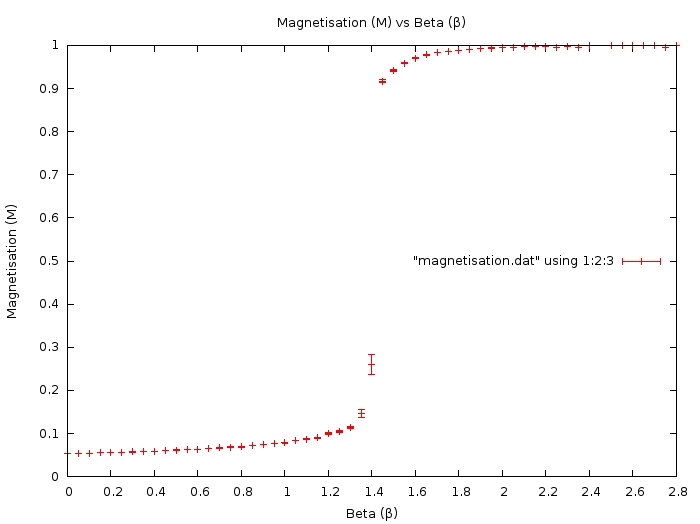
\includegraphics[width=\textwidth]{Q10MagnetisationBeta16x16RangeofBeta.png}
\end{figure}
\end{frame}

\begin{frame}{Specific Heat}
\begin{figure}
\centering
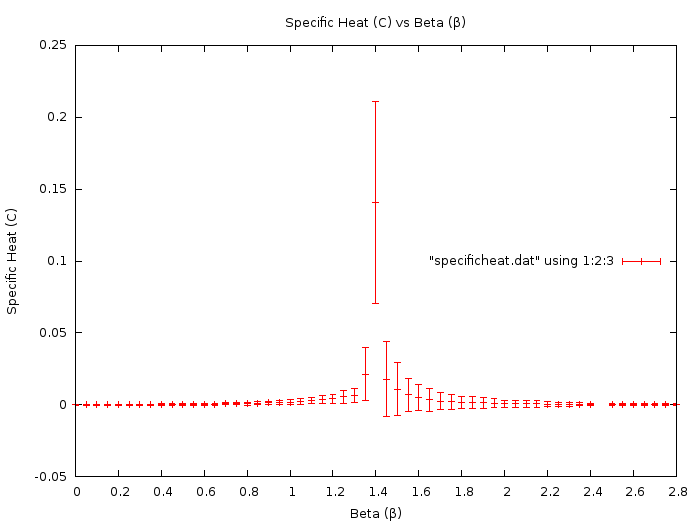
\includegraphics[width=\textwidth]{Q10SpecificHeatBeta16x16RangeofBeta.png}
\end{figure}
\end{frame}

\begin{frame}{Magnetic Susceptibility}
\begin{figure}
\centering
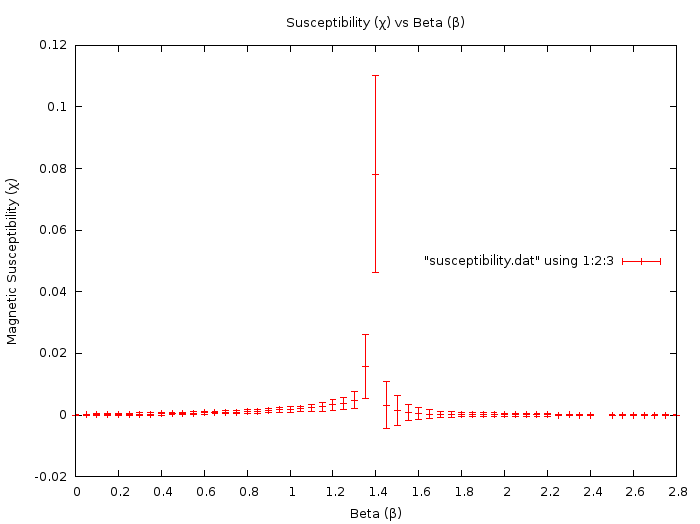
\includegraphics[width=\textwidth]{Q10SusceptibilityBeta16x16RangeofBeta.png}
\end{figure}
\end{frame}

\section{The Wang Landau Algorithm}
\begin{frame}{The Wang Landau Algorithm}
The Wang Landau algorithm provides a method to numerically calculate the Density of States.

By sampling across a restricted energy band whose width is determined by the Grid Size you can sample the value of $a_n$ for any Energy.

This measured quantity, $a_n$, is equivalent to the gradient of the Density of States and upon adding a continuity condition you can extract g(E).

$a_n$ is iterative and takes the form
\begin{equation}
a_{n+1} = a_n + \frac{12}{4L+L^2}\langle E^\star \rangle
\end{equation}

\end{frame}

\begin{frame}{The converging behaviour of $a_n$}
The behaviour for $a_n$ is such that it should converge rapidly upon it's value at each target point. A plot is provided below.
\begin{figure}
\centering
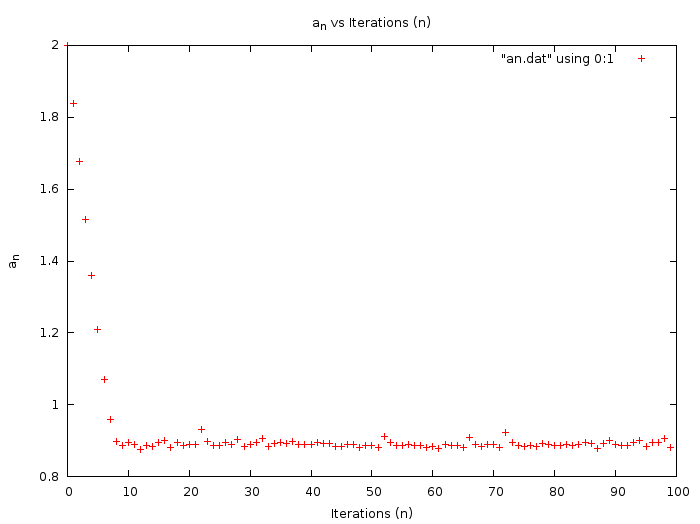
\includegraphics[width=0.7\textwidth]{An16x16Convergence.png}
\end{figure}

\end{frame}


\begin{frame}{Verifying the Wang Landau Results}

To verify the results returned from the Wang Landau I took the results from the Metropolis algorithm for the Energy at $\beta_c = \ln{(1+\sqrt{Q})}$.

It is impossible to perform a measurement for the thermodynamic limit. All computational tools would be unable to perform calculations and measurements for an infinite lattice.

To solve this problem I took a linear fit of the results to the thermodynamic limit instead.
\end{frame}

\begin{frame}{Q2 Verification}
\begin{figure}
\centering
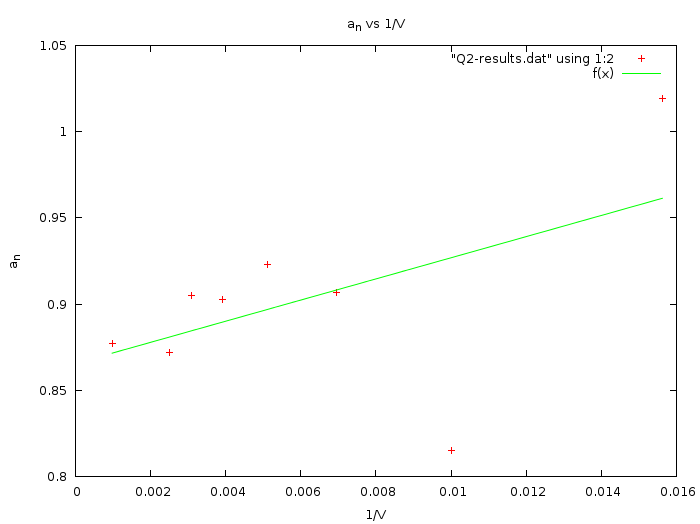
\includegraphics[width=\textwidth]{Q2-Verification.png}
\end{figure}
\end{frame}

\begin{frame}{What did I just see?}

What you just saw was the results of the Wang Landau algorithm for the Potts Model at the critical Energy for a variety of Grid Sizes against the inverse volume.
The fitted values and the theoretical results are shown below.
\begin{table}[H]
\centering
\begin{tabular}{|c|c|c|c|}
\hline
Q  & Theoretical & Result   & Error    \\ \hline
2  & 0.881373587 & 0.865616 & 0.03173  \\ \hline
3  & 1.005052539 & 0.996294 & 0.01123  \\ \hline
4  & 1.098612289 & 1.11538  & 0.002026 \\ \hline
8  & 1.342454046 & 1.34759  & 0.008933 \\ \hline
10 & 1.426062439 & 1.43679  & 0.0152   \\ \hline
\end{tabular}
\caption{All of the results match the Theoretical within Error}
\end{table}

\end{frame}

\begin{frame}{Sampling $a_n$ across Energy Bands}
As described earlier, the different energies of the system can be broken down into specific energy bands.
When sampling $a_n$ across all of these bands you get the resulting plot.
\begin{figure}
\centering
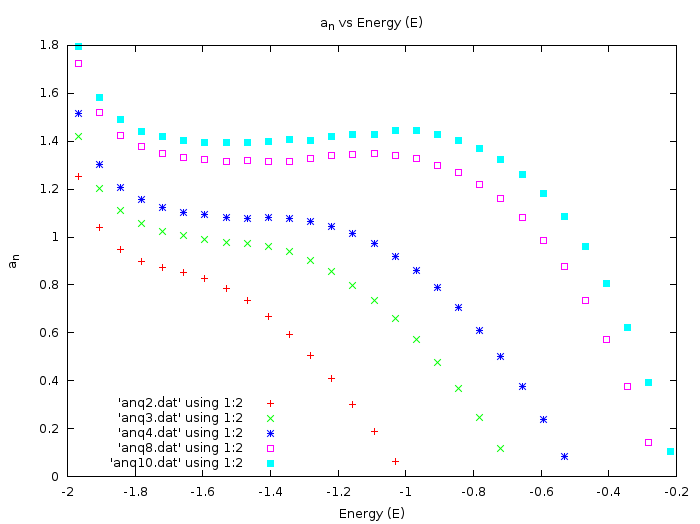
\includegraphics[width=0.7\textwidth]{a_n-rescaled.png}
\end{figure}
\end{frame}

\begin{frame}{Reconstructing the Density of States}
Taking the results from the energy band sampling of $a_n$ and applying a continuity condition on the locally linear approximation you get the continuous Density of States.
\begin{figure}
\centering
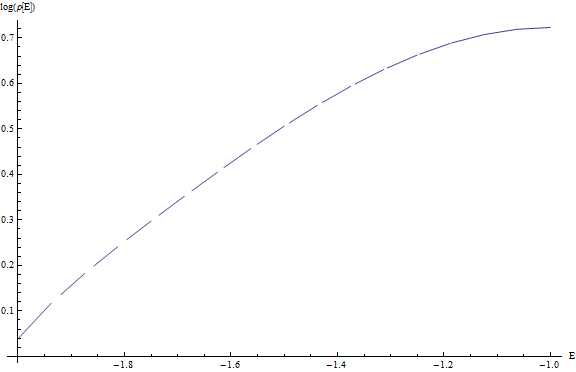
\includegraphics[width=0.75\textwidth]{Q2Log(g(E)).png}
\end{figure}
\end{frame}

\begin{frame}{The Interface Free Energy and Tensions}

We now have the necessary information to calculate the Interface Tensions.

\begin{equation}
Z = \int g(E) e^{-\beta E} dE
\end{equation}
\begin{equation}
F_I (L) = -log \frac{\tilde{Z}(L)}{Z(L)} - log(L)
\end{equation}
\begin{equation}
\sigma = \lim_{L \to \infty} \frac{F_I(L)}{L^{D-1}}
\end{equation}

The graphs showing the behaviour of the Interface Tensions are given on the next slide.

\end{frame}

\begin{frame}{Q2 Interface Tension at the Thermodynamic Limit}

\begin{figure}
\centering
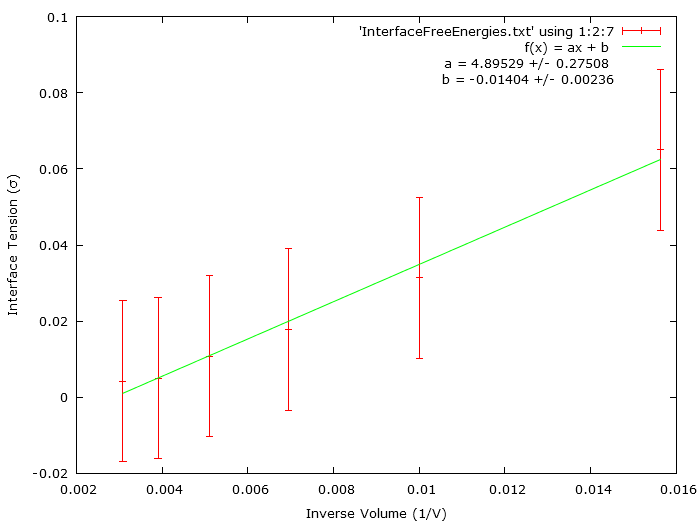
\includegraphics[width=0.75\textwidth]{Q2-InterfaceTension.png}
\end{figure}

\end{frame}


\begin{frame}{Q2 Interface Tensions against $\beta$ for Various Grid Sizes}

\begin{figure}
\centering
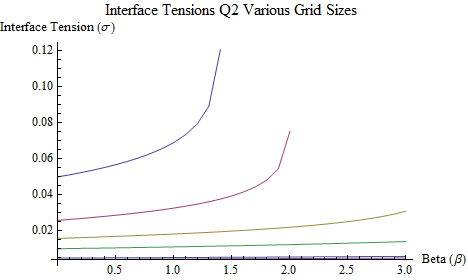
\includegraphics[width=0.75\textwidth]{Q2VariousGridSizesTensions.png}
\end{figure}
\end{frame}

\section{Summary}
\begin{frame}{Summary}
At the beginning of the presentation, I started out with the goal of introducing you to the points on the list below.
\begin{enumerate}
	\item An introduction to the Potts Model
	\item Accessing Thermodynamic quantities
	\item Why do we care about Interfaces
	\item How to add a twist
	\item Project Results
\end{enumerate}

\begin{center}
\large{Thanks for listening.}
\end{center}
\end{frame}

\end{document}